\documentclass{sigchi}

\usepackage{balance}  % to better equalize the last page
\usepackage{graphics} % for EPS, load graphicx instead
\usepackage{times}    % comment if you want LaTeX's default font
\usepackage{url}      % llt: nicely formatted URLs

\toappear{}

\graphicspath{{graphics/}} 

% llt: Define a global style for URLs, rather that the default one
\makeatletter
\def\url@leostyle{%
  \@ifundefined{selectfont}{\def\UrlFont{\sf}}{\def\UrlFont{\small\bf\ttfamily}}}
\makeatother
\urlstyle{leo}

% To make various LaTeX processors do the right thing with page size.
\def\pprw{8.5in}
\def\pprh{11in}
\special{papersize=\pprw,\pprh}
\setlength{\paperwidth}{\pprw}
\setlength{\paperheight}{\pprh}
\setlength{\pdfpagewidth}{\pprw}
\setlength{\pdfpageheight}{\pprh}

% Make sure hyperref comes last of your loaded packages, 
% to give it a fighting chance of not being over-written, 
% since its job is to redefine many LaTeX commands.
\usepackage[pdftex]{hyperref}
\hypersetup{
  pdftitle={Fitness Adventure: an interactive floor game to maintain body fitness},
  pdfauthor={LaTeX},
  pdfkeywords={HCI, fitness, floor, adventure},
  bookmarksnumbered,
  pdfstartview={FitH},
  colorlinks,
  citecolor=black,
  filecolor=black,
  linkcolor=black,
  urlcolor=black,
  breaklinks=true,
}

% create a shortcut to typeset table headings
\newcommand\tabhead[1]{\small\textbf{#1}}

% End of preamble. Here it comes the document.
\begin{document}

  \title{Fitness Adventure: an interactive floor game to maintain body fitness}

  \author{
    \alignauthor Carl Ambroselli, Marc-Philipp Bismar, Marvin Bornstein, Julius Treike\\
    \affaddr{Hasso-Plattner-Institut}\\
    \affaddr{Potsdam, Germany}\\
    \email{\{carl.ambroselli, marc-philipp.bismar, marvin.bornstein, julius.treike\}@student.hpi.de}
  }

  \maketitle

  \begin{abstract}
    We introduce a jump 'n' run game for interactive floors to maintain body fitness. Players control themselves directly by stepping, jumping or lying on the floor. In a forest, users jump over fallen trees or cross an ocean by holding themselves on ice floes. Repairing a bridge in shortage of time or similar complex tasks pack fitness exercises in an exciting adventure. This motivates users to do regular physical activity.
  \end{abstract}

  \section{Introduction}
    Most of today's tasks are done by machines. The majority of people spend almost the whole day in an office -- sitting.
    Fitness apps for smartphones are getting more and popular and many people subscribe to local fitness centers. 
    At least, the persons we asked about their sports activity in our contextual inquiry. 

    \begin{figure}[ht]
      \centering
      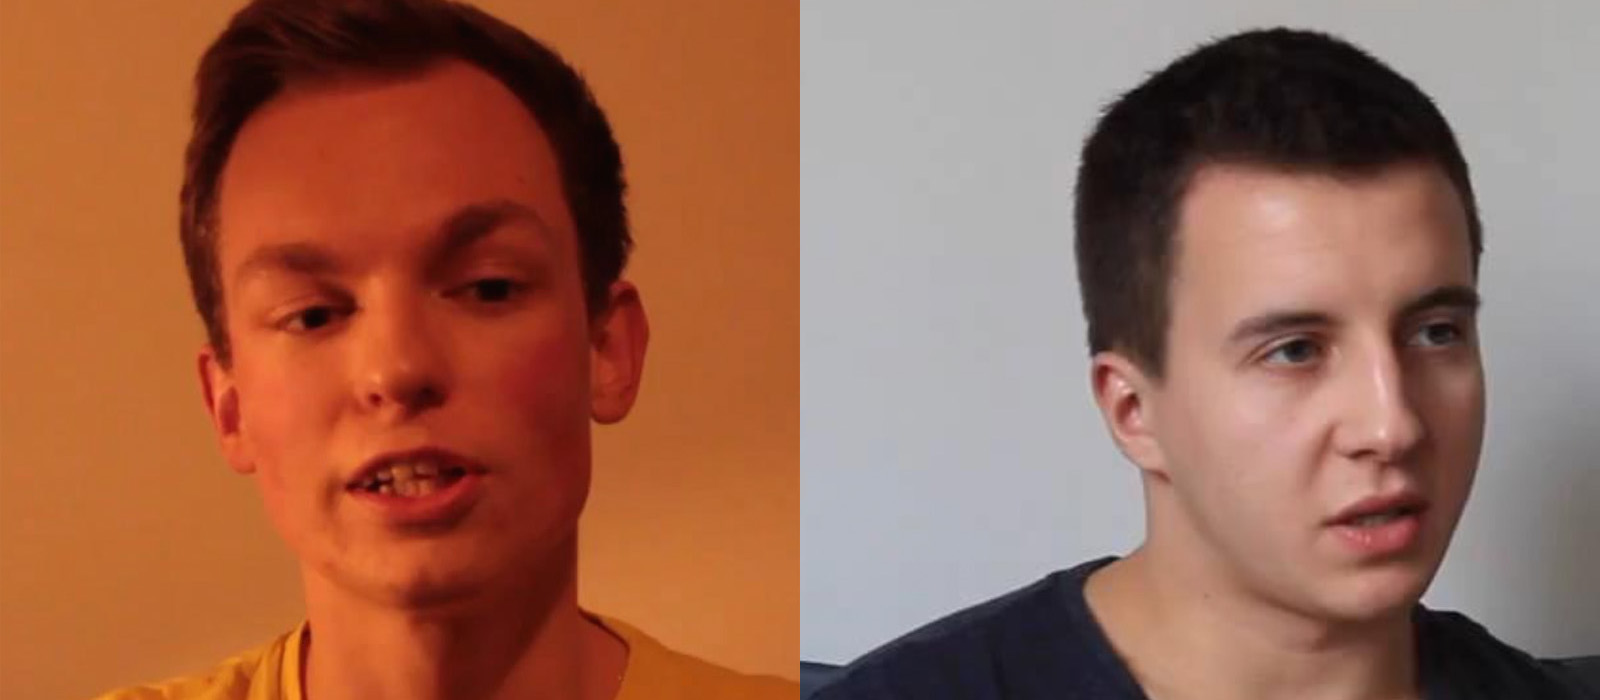
\includegraphics[width=\columnwidth]{users_casual}
      \caption{Interviewees with casual sports background. Justus Wirth (left) and Markus Petrykowski (right)}
      \label{fig:users_casual}
    \end{figure}

    \begin{figure}[ht]
      \centering
      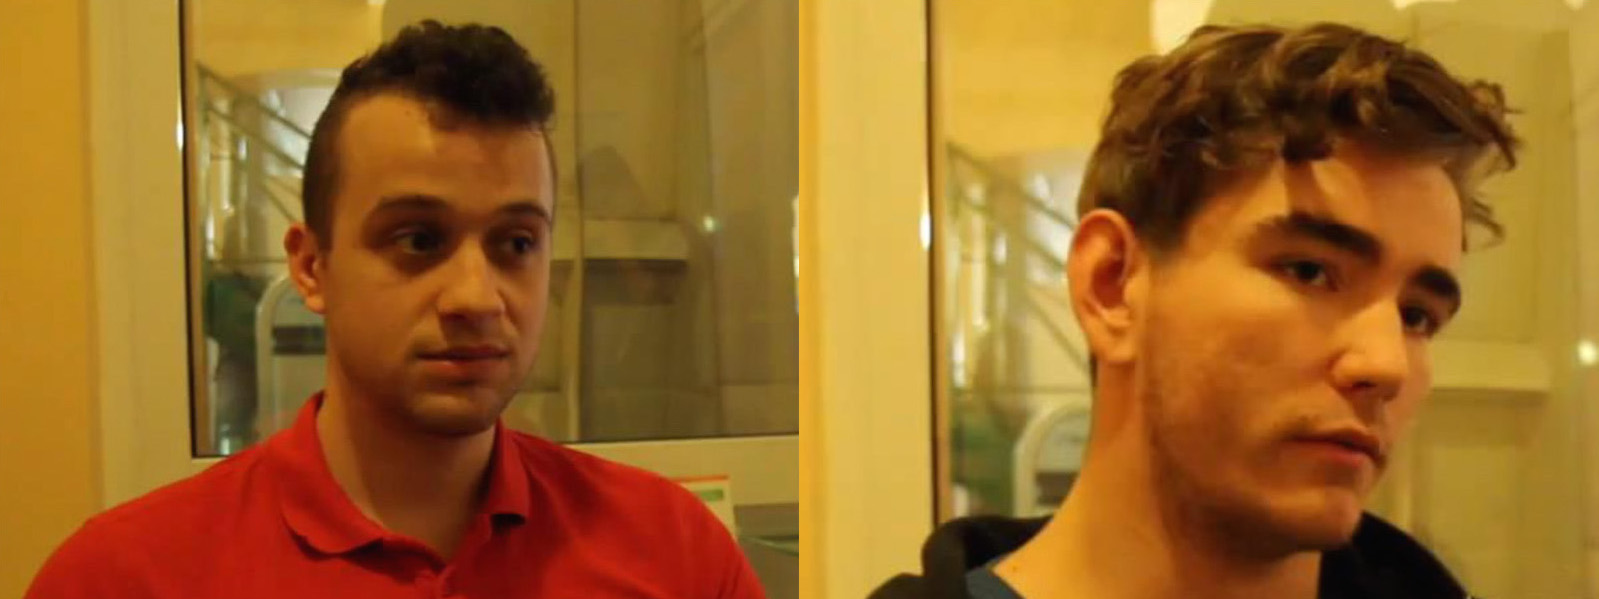
\includegraphics[width=\columnwidth]{users_pro}
      \caption{Interviewees with professional sports background. Ruben Zieger (left) and Carl Link (right)}
      \label{fig:users_pro}
    \end{figure}

    Markus (Figure \ref{fig:users_casual} on the right) studies computer science in Potsdam and has not much time for doing sport. In order to be balanced and healthy, he goes swimming or climbing once a week. He wants a flexible, non-complex and short exercise pack. A notable training progress would be a great motivation.

    Justus Wirth (Figure \ref{fig:users_casual} on the left) started doing freeletics in order to maintain health and get his body in shape. He wants to improve his performance in every training session and somehow get feedback on how well he performed his exercises.

    Carl and Ruben (Figure \ref{fig:users_pro}) from the \emph{Fit in Friedrichshain} fitness centre do bodybuilding on a professional level. Their motivations consists also of their bodies as well as of their jobs. In general, the motivation depends on the individual person. Their clients, however, already bring the necessary motivation for training. Both, Carl and Ruben, were very interested in the idea of a ``touch floor exercising application'', but mentioned problems regarding gym equipment. ``\emph{Every kind of activity is good}'' says Carl, ``\emph{but there are no effective exercises for training the shoulders for example}''. 

  \begin{figure}[!t]
    \centering
    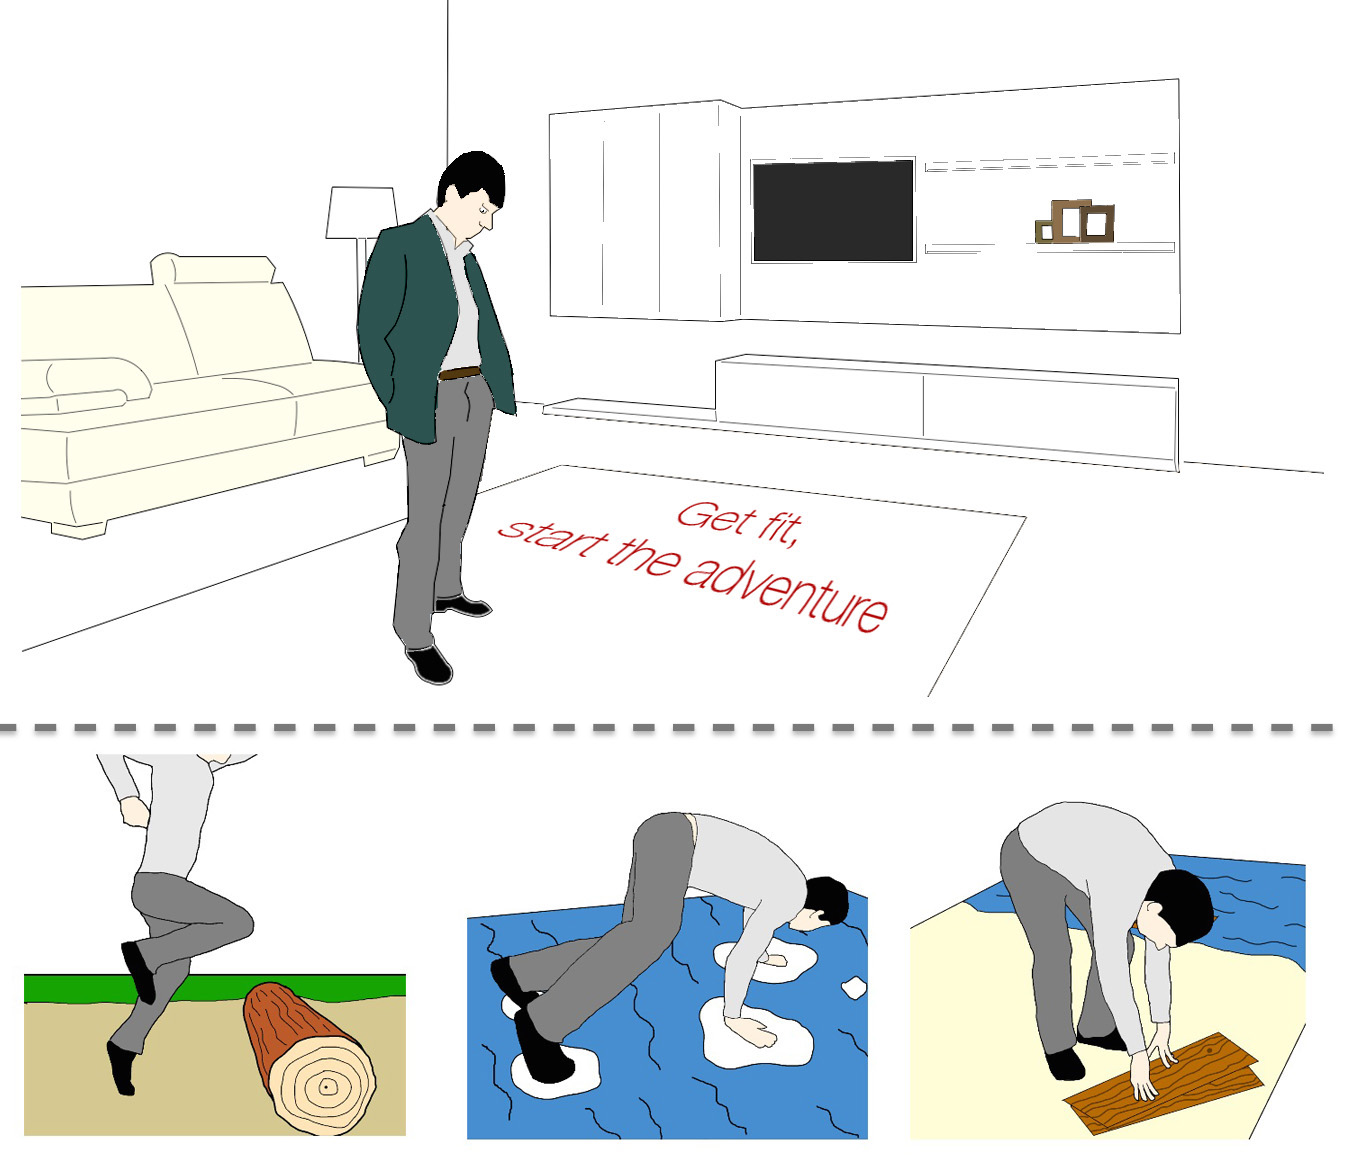
\includegraphics[width=\columnwidth]{roto_main_2}
    \caption{doing sport exercises as part of the game on an interactive floor}
    \label{fig:figure1}
  \end{figure}

    As a result, we focus on regular activity, instead of building up muscles and offer another approach to motivate activity: a video game. Users embody the protagonist themselves, explore the world and beat their own highscores by completing the level faster. This enables users to improve on every ``\emph{training session}'' and also requires more energy and endurance. In addition, the game offers another environment for exercises than the traditional fitness studio and thus addresses other kinds of people.


\section{Walk-through}

  \subsection{Old Forest: the first territory in the game} % (fold)
  
    \begin{figure}[htb]
      \centering
      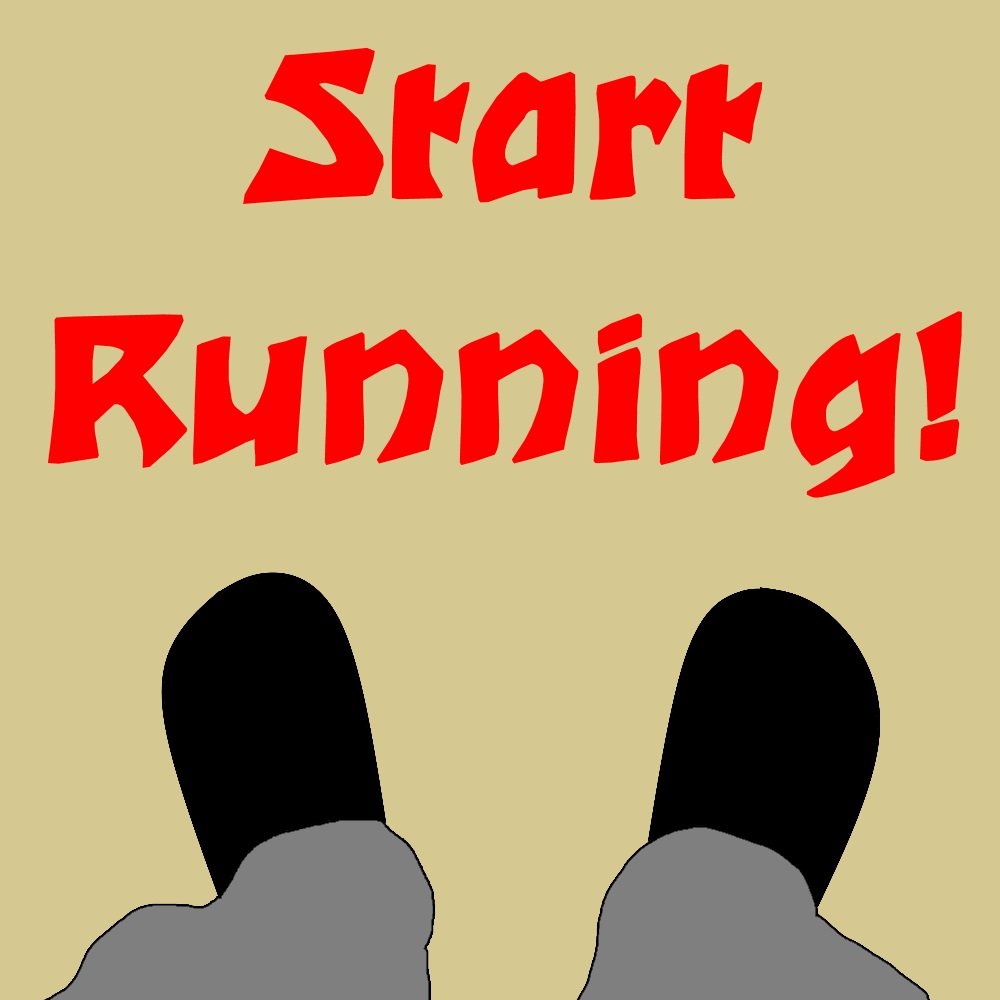
\includegraphics[width=0.32\linewidth]{Image_4.jpg}
      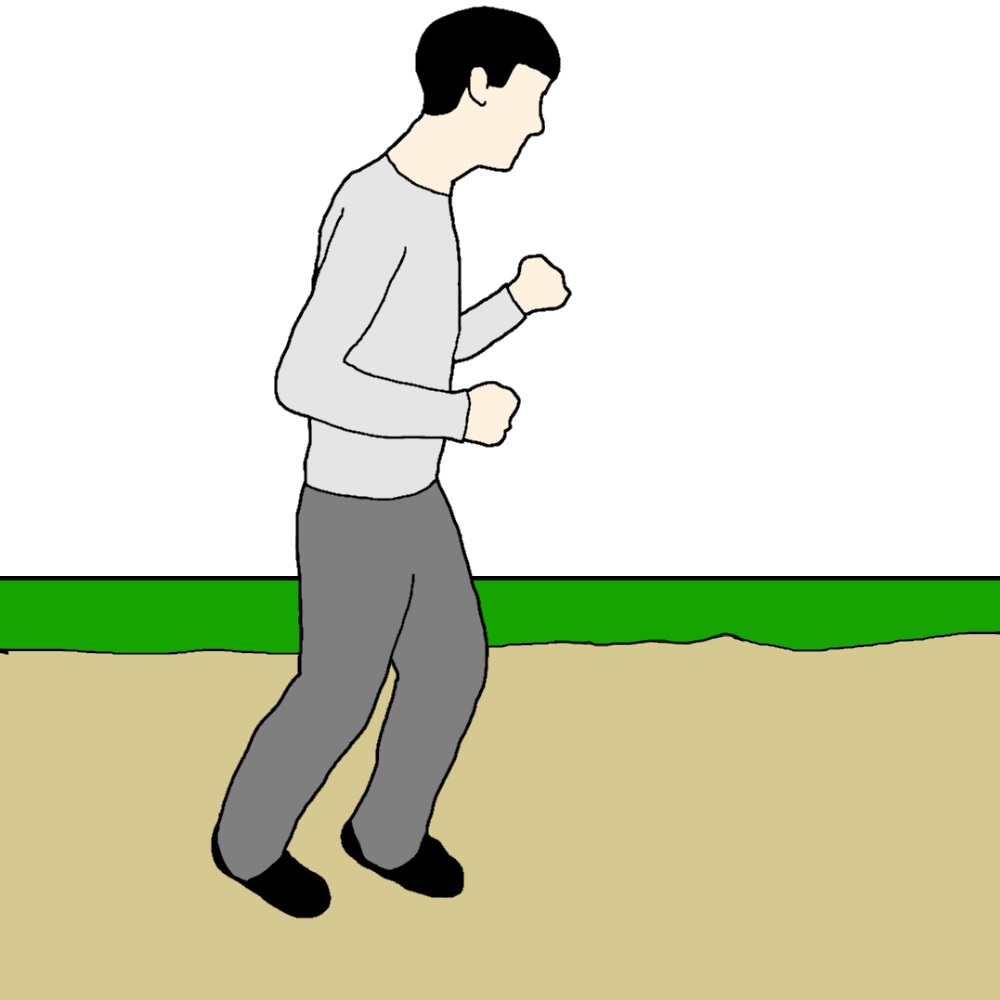
\includegraphics[width=0.32\linewidth]{Image_5.jpg}
      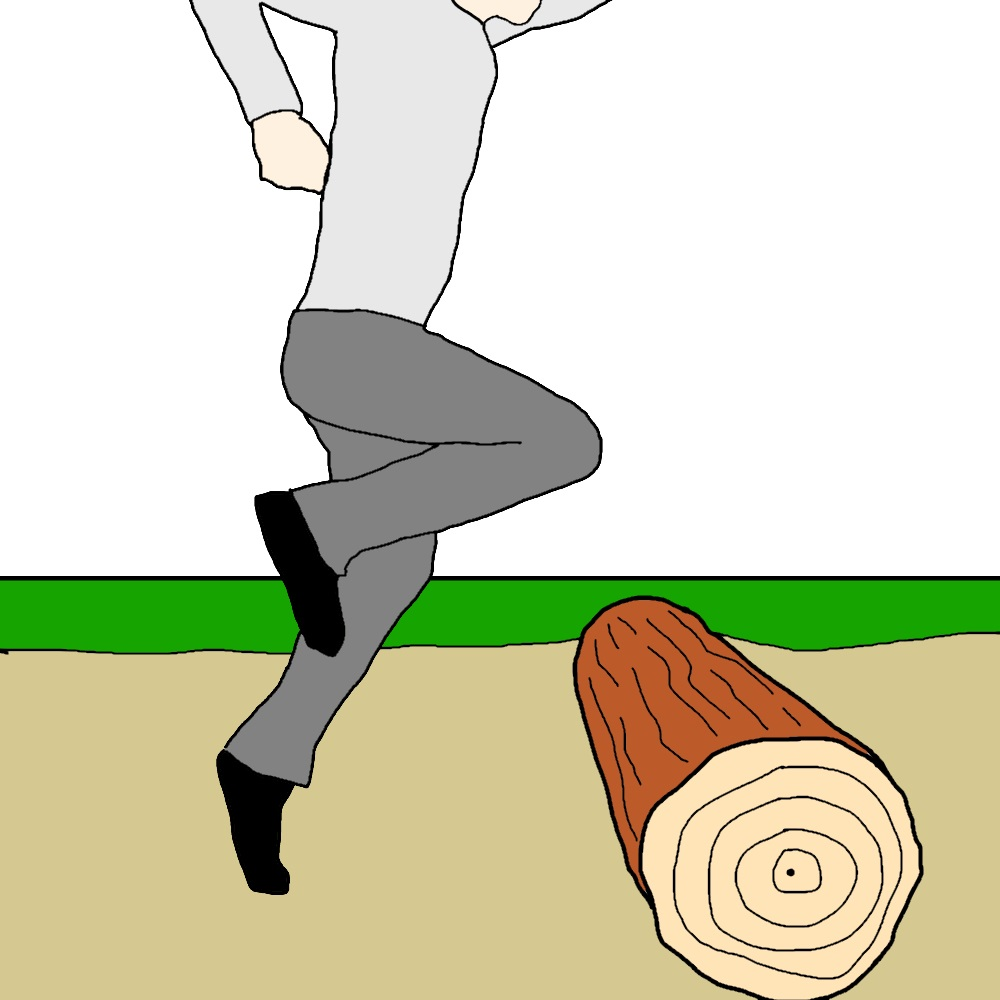
\includegraphics[width=0.32\linewidth]{Image_1.jpg}
      \caption{(left) Enter the floor to start the game. (middle) Step on the spot to move through the world. (right) Jump over fallen trees.}
      \label{fig:start}
    \end{figure}

    In this scenario, the student Andy wants to do his regular activity and get exhausted. The specific task is about to raise his heart rate over 180. Therefore, Andy enters the floor and it tells him to start running (see figure \ref{fig:start} on the left). Andy now steps on the spot and the ground under his feet moves along (figure \ref{fig:start}, in the middle). Whenever he meets a fallen tree, he has to jump over it (figure \ref{fig:start}, on the right). This does not need any explanation, since nobody can walk through a tree. If he does this anyway, he will receive a time penalty of 10 seconds (figure \ref{fig:penalty}, on the left and in the middle).

  \subsection{Arctic Sea: the second territory in the game} % (fold)

    \begin{figure}[htb]
      \centering
      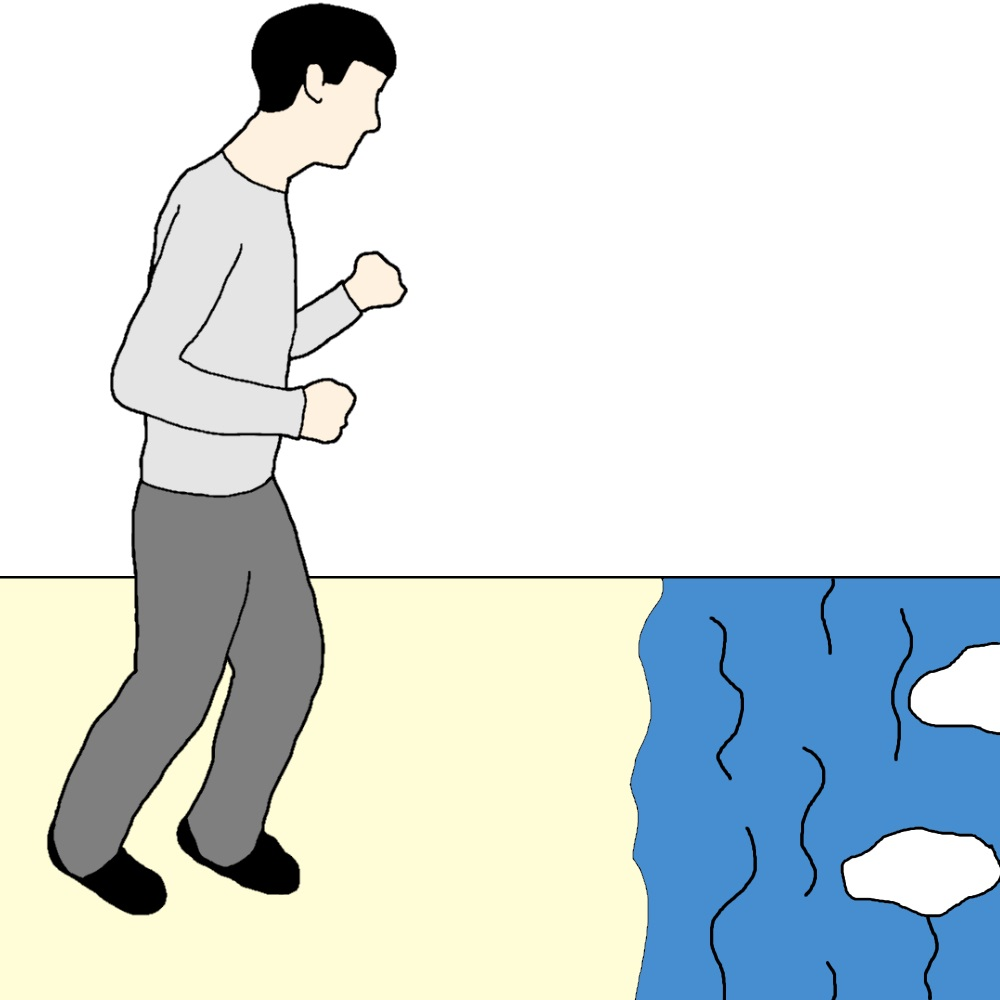
\includegraphics[width=0.32\linewidth]{Image_7.jpg}
      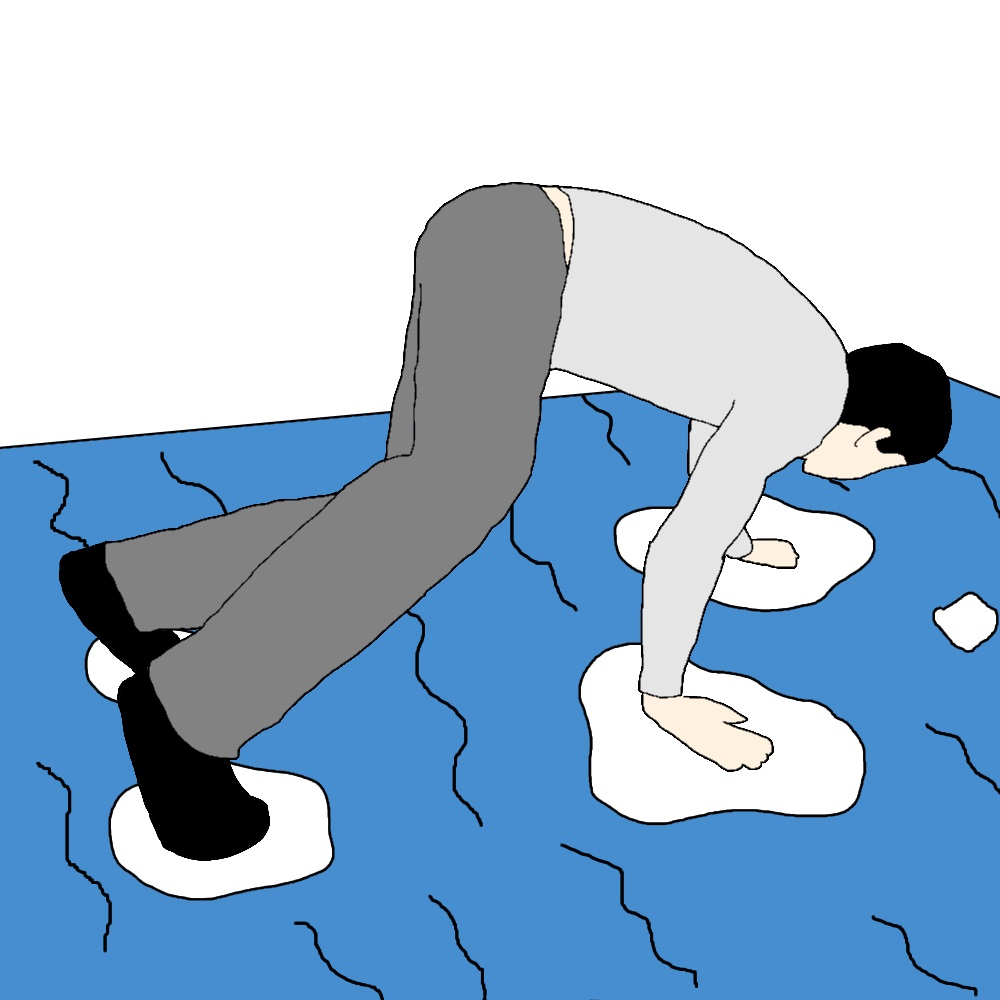
\includegraphics[width=0.32\linewidth]{Image_2.jpg}
      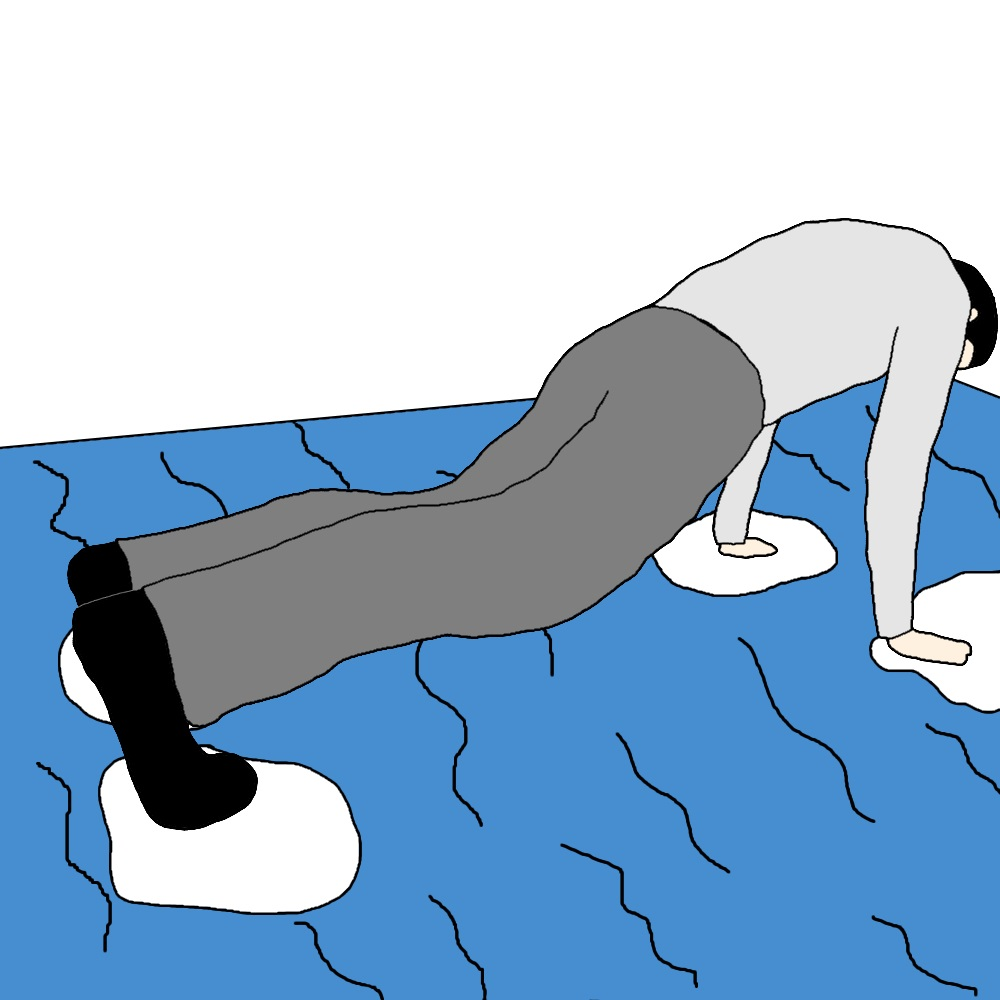
\includegraphics[width=0.32\linewidth]{Image_8.jpg}
      \caption{(left) Reach the sea. (middle) Hold on ice floes to get over. (right) Ice floes will sink, so always switch to a stable one.}
      \label{fig:ice_floe}
    \end{figure}

    After running for a while, Andy will reach the sea. He can obviously not cross it (figure \ref{fig:ice_floe}, on the left). He notices ice floes appearing. He can drift over the water by holding himself on those ice floes (figure \ref{fig:ice_floe}, in the middle). The ice floes sink and melt because of the weight and the warm hands. They begin to get smaller and smaller. Andy has to move from ice floe to ice floe in his position. He does not want to fall into the cold water (figure \ref{fig:ice_floe}, on the right). If he does anyway, he will receive a time penalty of 10 seconds (see again figure \ref{fig:penalty}, the right image).

  \begin{figure}[htb]
    \centering
    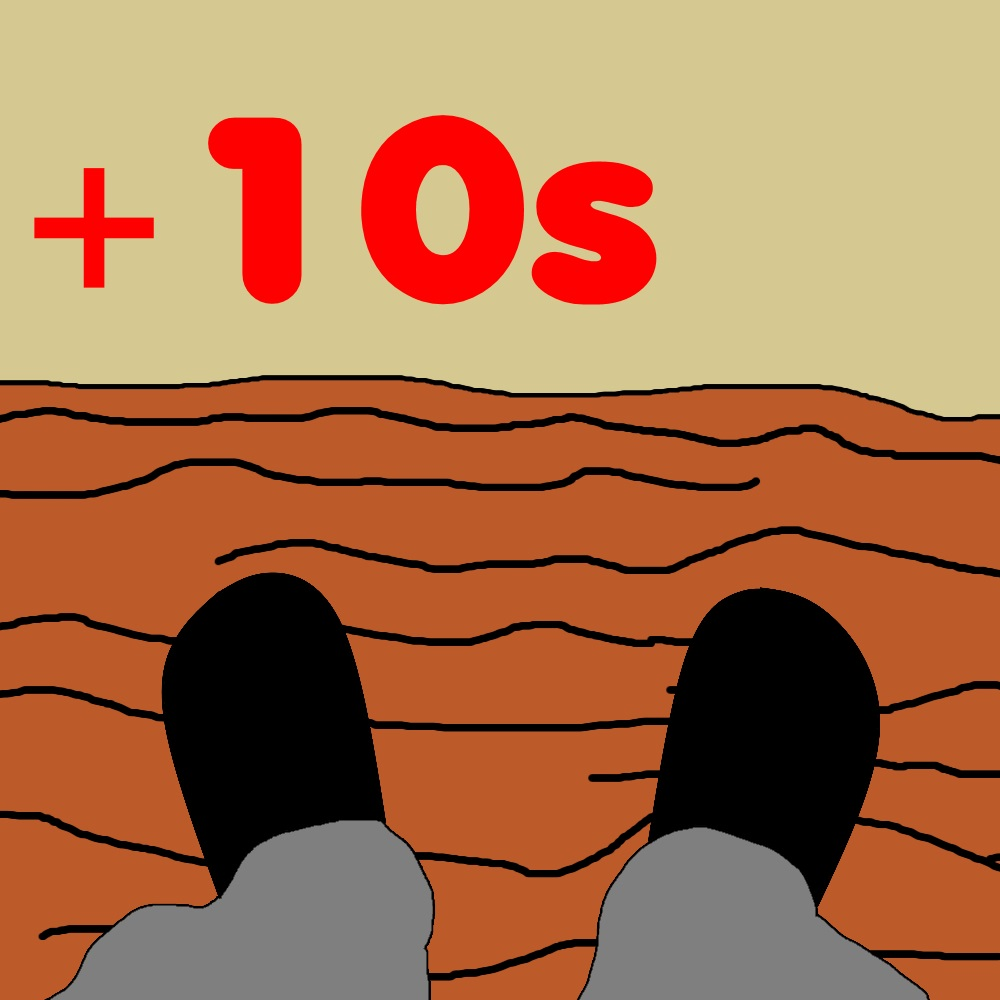
\includegraphics[width=0.32\linewidth]{Image_6.jpg}
    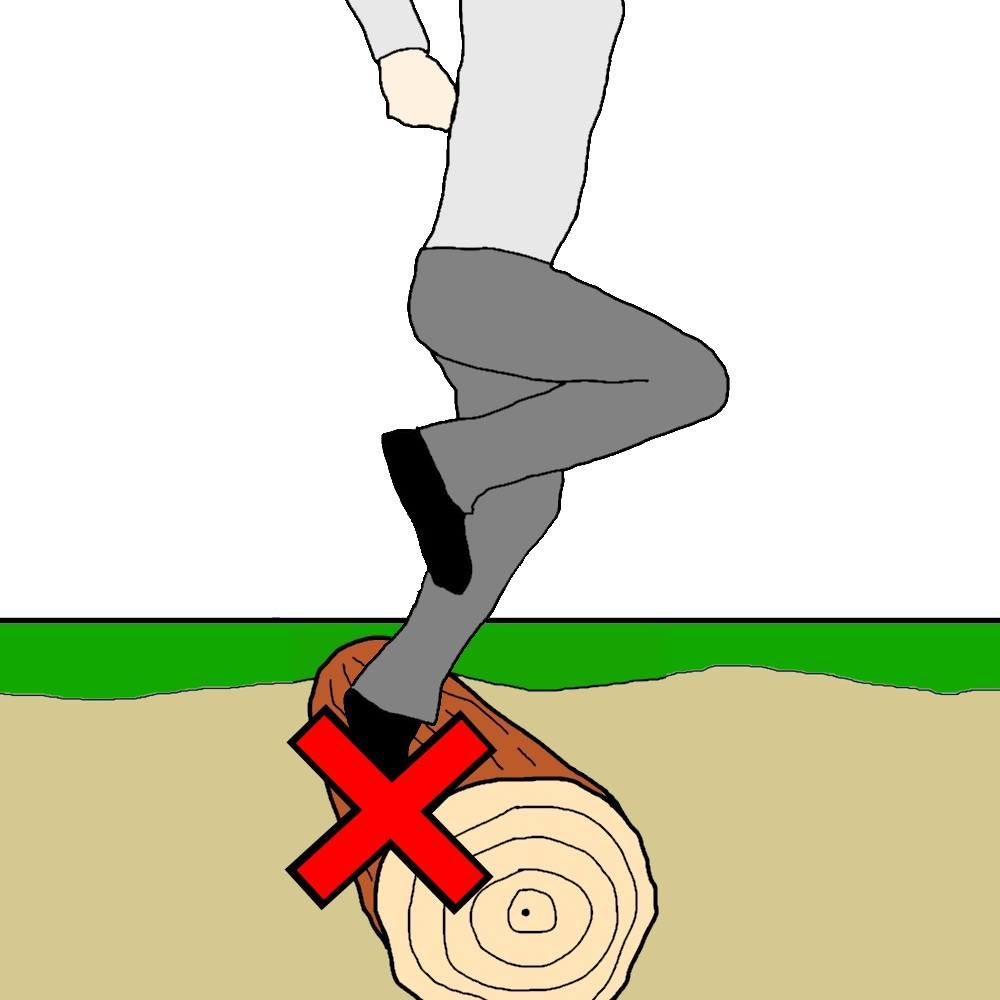
\includegraphics[width=0.32\linewidth]{Image_15.jpg}
    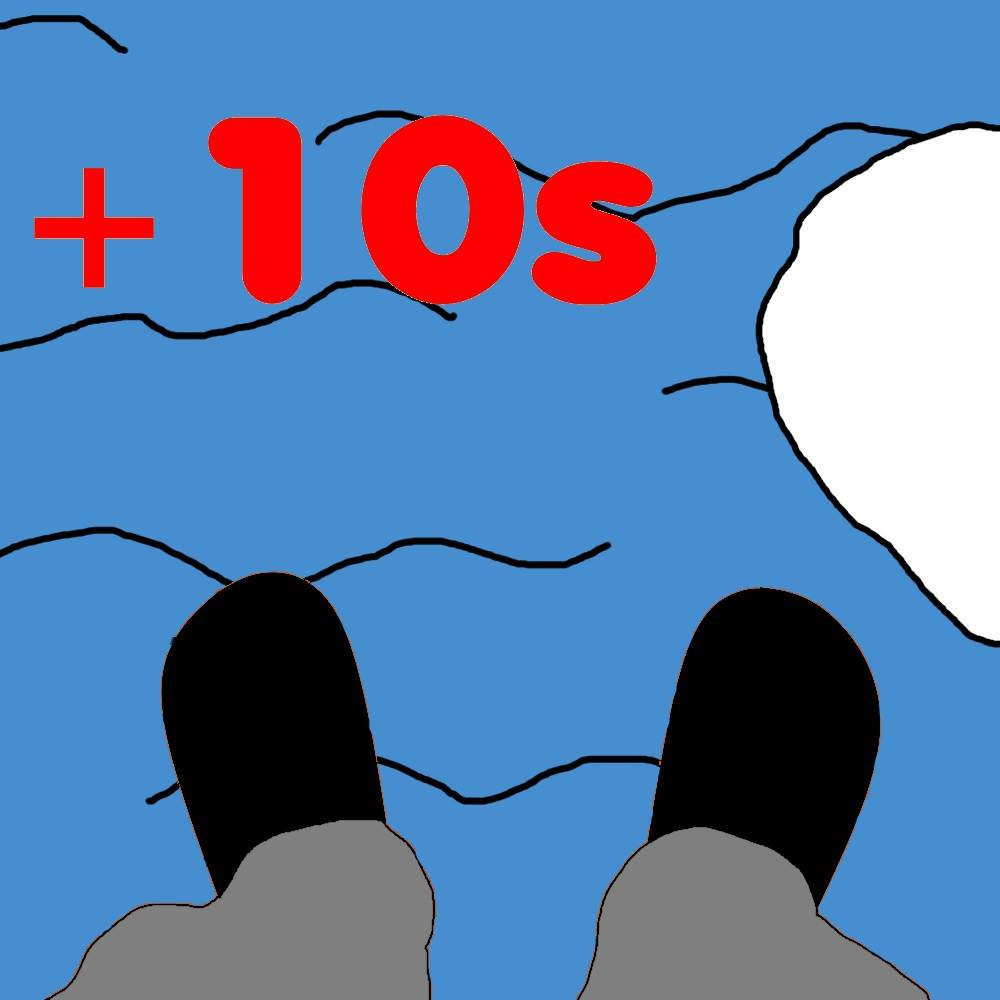
\includegraphics[width=0.32\linewidth]{Image_16.jpg}
    \caption{Penalty: (left) Hitting a tree brings 10s time penalty. (middle) Illustration from the side. (right) Touching the water does as well.}
    \label{fig:penalty}
  \end{figure}

  \subsection{Workout World: repeating territories} % (fold)
  
    When Andy finally arrives at a beach again, he can run further. Depending on the world, he will run through the forest (described in subsection \emph{Old Forest}) and drift over the sea (described in subsection \emph{Arctic Sea}) some more times. This is how the world looks like. There are some areas with different kinds of activities that create a workout together. The same applies to the third territory, the broken bridge. 

  \subsection{Broken Bridge: the third territory in the game} % (fold)

    \begin{figure}[htb]
      \centering
      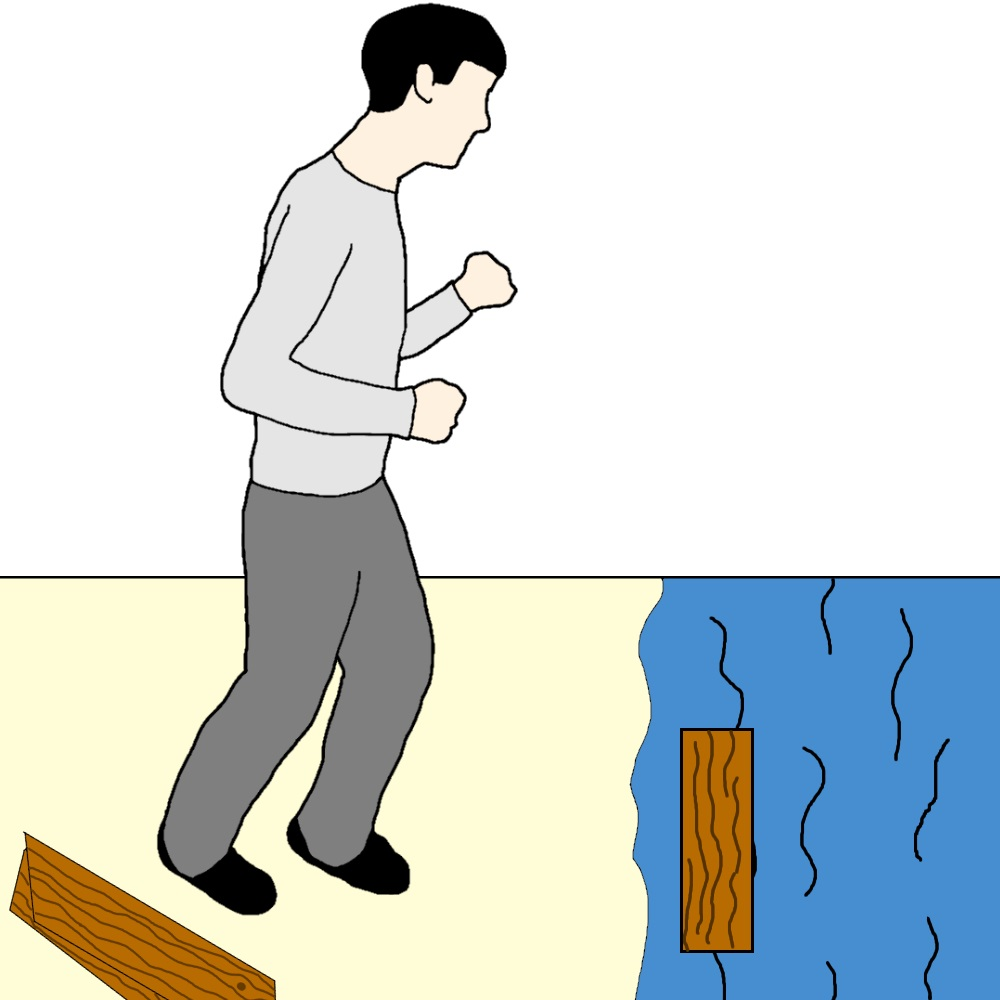
\includegraphics[width=0.32\linewidth]{Image_9.jpg}
      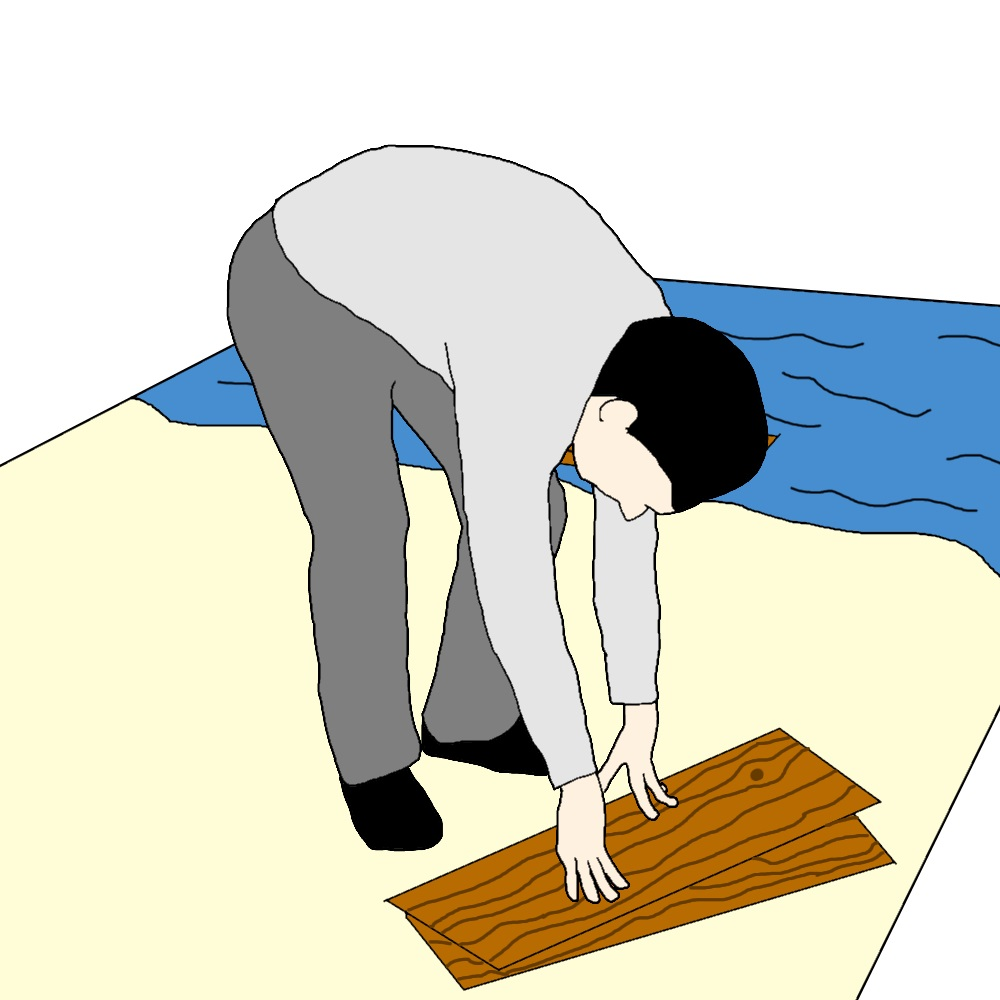
\includegraphics[width=0.32\linewidth]{Image_3.jpg}
      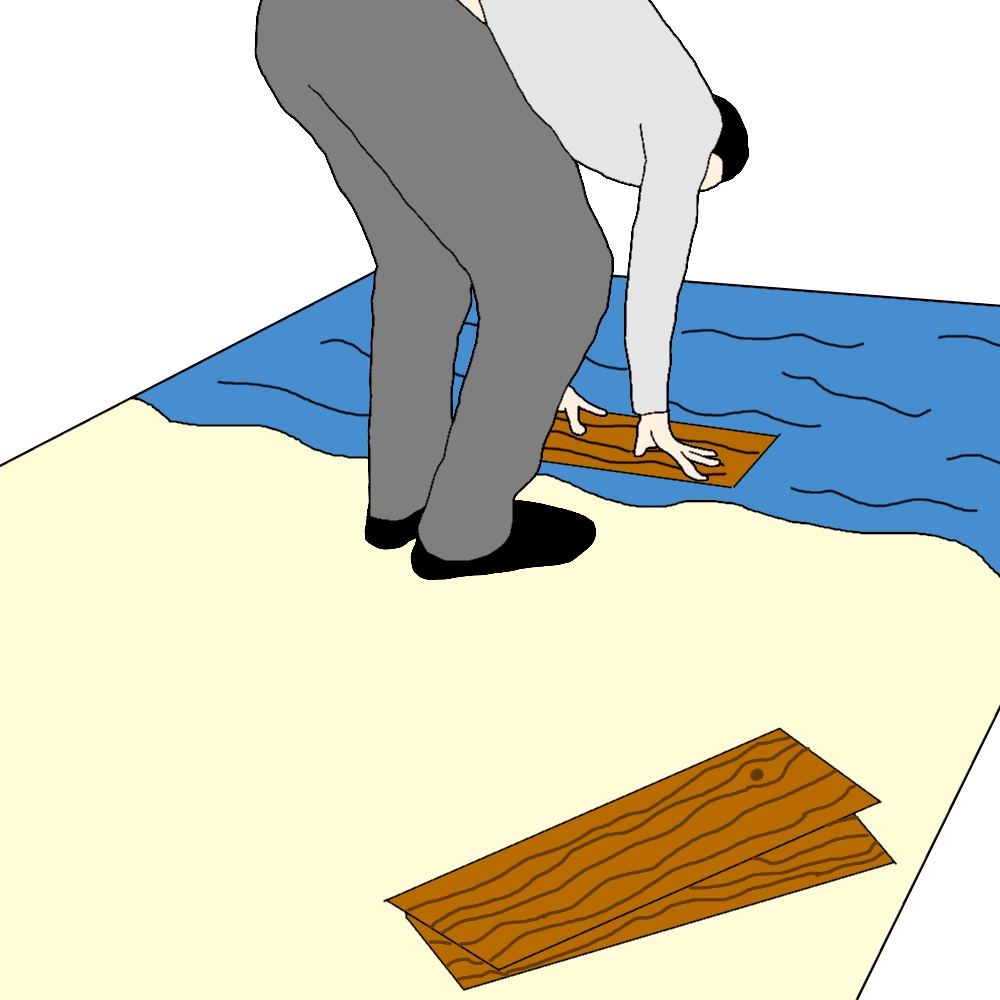
\includegraphics[width=0.32\linewidth]{Image_10.jpg}
      \caption{(left) Reach a broken bridge. (middle) Get the wooden planks. (right) Build up the bridge to cross the water. (Remember penalty)}
      \label{fig:bridge}
    \end{figure}

    Andy now arrives at a river. He can see a bridge, but it is broken. He looks around and finds wooden planks. He now repairs the bridge with the wooden planks by alternately touching the wooden planks and the broken bridge. Therefore he has to repeatedly run between the planks and the bridge. This includes accelerating, stopping and bending down. Once the bridge is repaired, Andy can pass the river and continue his adventure.

  \section{Workout Result: what the user has achieved} % (fold)
  \label{sec:section_name}
  
    \begin{figure}[htb]
      \centering
      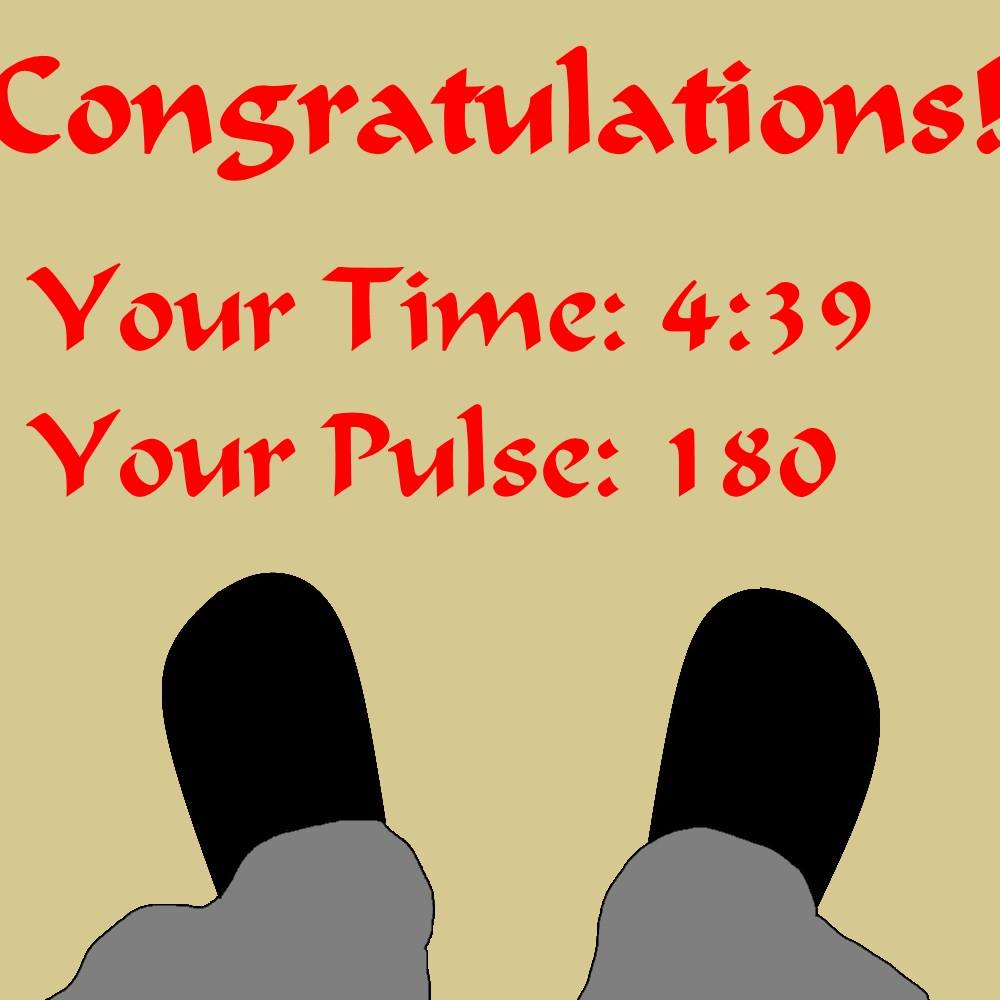
\includegraphics[width=0.32\linewidth]{Image_17.jpg}
      \caption{Final screen; shows the time the user needed to run through the world and the heart rate, if the hardware is available. The user is also congratulated, because he finished the workout.}
      \label{fig:end}
    \end{figure}

    When Andy has run through the world, he will see the final screen. It contains the needed time and his heart rate, as well as a congratulation. The next time, he can try to beat his record. This would require him to step and repair the bridge much faster. 

\section{Design}

  \subsection{Use the complete screen space during workout} % (fold)
  \label{sub:use_the_complete_screen_space_during_workout}

    A first approach to provide the workout functionality to the user was to show three fitness mats, each offering several exercises for training certain body parts: a warm-up, an ``arms training'' and a ``legs training'' mat. The idea was that using our application assures right performance of the exercises and a balanced workout by recommending a workout plan to the user. This would have been done by briefly introducing every exercise. 

    So the training would always start with a warm-up and then give the user the freedom to choose every following exercise. During contextual inquiry we found out that the majority of users did not get why there were three different mats for one person. Furthermore it was unnecessarily inconvenient to display workout instructions on a third of the screen, so we scraped the idea of multiple fitness mats to use the whole screen for guiding the users.

  \subsection{Motivate the user with game elements } % (fold)
  \label{sub:motivate_the_user_with_game_elements_}

    One of the most challenging requirements when designing a fitness application is to keep up the user's motivation. When first conceiving a full screen application we tried to fulfill this with a different exercise choosing menu which should fasten the choosing process. To start training, the user had to tap one of sundry bubbles, floating around on the screen. Each contained a small illustration of an exercise combined with the designation of either a time span or repetitions. However, in our paper prototype study two out of three participants did not even know what the exercises were about, but time pressure turned out to be an actuating game concept perfectly matching our demands. From now on the passed time always would be displayed to the user during a workout. But still we had to solve the issue, that fitness exercises are not commonly known amongst the users.

  \subsection{Dictate Exercises with game elements } % (fold)
  \label{sub:dictate_exercises_with_game_elements_}

    We needed to find a way to instruct a user to perform an exercise without expecting him to know it. This means, that every exercise the user would chooses had to be explained or shown first. Within task analysis, we noticed that this violates the need for a short workout, because much time is spent on selecting and explaining workouts. So we decided to not let the user choose a preferred exercise anymore, but transfer him in a virtual environment of which the user's tasks directly come out, as shown in the walk-through. This virtual environment would be a path to run along. For instance when the user runs and a tree appears he automatically get, that he has to overcome this obstacle by jumping. This way there are even less instructions necessary and no time is spent on choosing a workout anymore. Adding these further game elements also turned out to provide more fun.

  \subsection{Penalties during workout, rewards after workout} % (fold)
  \label{sub:penalties_during_workout_rewards_after_workout}

    During further progress we tested whether punishing or rewarding leads to better workout results. In a first approach the users were rewarded by time reduction for each correctly performed exercise. But as exercises like jumping over a tree are quite fast done, a first test user was rewarded more than one time a second, so that both the motivation effect was gone and the time reduction made no sense anymore. Furthermore the exercises the user has to perform are quiet simple so that a false performance is more unlikely than a correct one. And as we don't want the user to be permanently distracted by penalties or rewards, we decided to punish false performances. The motivating reward was now to finish a workout faster than before or beat a time of another user.

  \subsection{Instantly start game } % (fold)
  \label{sub:instantly_start_game_}

    We had several iterations concerning when to start the game. From contextual inquiry we learned, how important a good warm-up is, which is why we kept the concept of always starting with a warm-up this far. But in the paper prototype study, the users did not get, why they were forced to do a warm-up and could not start immediately. So we left it out, as it was not necessary for this kind of game anymore. In the final version we chose to start the game as soon as someone starts running on the floor to provide the simplest solution as possible. During heuristic evaluation we identified that there must be a short message telling the user that he should start running. From that point on he understood how to start a workout and make progress.

  \subsection{Use a fixed map} % (fold)
  \label{sub:use_a_fixed_map}

    One of the last design decisions we faced was whether to generate a unique map each run or use the same map every time. To vary the user's challenge varies from time to time, generating a map was the obvious approach. The problem was that the comparability of the times for a workout was not given anymore. But as we proofed the concept of motivation by time pressure earlier, we finally decided to use a fixed map, so that a user could compete with another user or himself.

\section{Conclusion}

  When designing applications for interactive floors, user studies and exploration with prototypes becomes extremely important since there are no patterns and the problem domain is yet unexplored. During the process, our evaluation of the users' needs changed radically. When asking users what they wanted they looked at existing solutions and tried to map them to the floor. If we followed those, we would have ended up with a fitness mat and a video player. This, however, is already an existing solution for people without any sport equipment. We collected important aspects from users: the need for motivation and limited free time. First we mapped them to possible exercises on the floor and later came to the conclusion, that games are the most interactive solution motivating users with fun when doing workouts. The ability to challenge your highscore, pushes your goals and visualize your progress. 

  Developing an interactive protoype for a floor requires a lot amount of work. Paper prototyping turned out to be a powerful tool in order to find flaws in our designs as users were able to imagine the system.

  Even when users want to do fitness activity with our application, they look for the simplest solution to solve a game. Therefore we need to design fitness games that forces users to do certain activity instead of giving them the freedom on how they want to solve a task.

  In the future, the game could also contain a map editor. This would satisfy the users need to configure their workout. In addition, it would make the game more interesting and diversified. There should also be some more territories containing new sport exercises. The users could have to jump a lot, or maybe lift another person.


\end{document}